\documentclass[10pt]{article}
\usepackage[utf8]{inputenc}
\usepackage[T1]{fontenc}
\usepackage{amsmath}
\usepackage{amsfonts}
\usepackage{amssymb}
\usepackage[version=4]{mhchem}
\usepackage{stmaryrd}
\usepackage{hyperref}
\usepackage{enumitem}
\usepackage{graphicx}
% \graphicspath{images/}
\begin{document}

\tableofcontents
\newpage
\section{Introduction}
A retrial queue consists of server(s) and a queue. Customers arrive according to a poisson process. These are called primary calls. If the server is free at the time of primary call, they start getting served immediately. Otherwise , they are added to the queue, and serve as a source of repeated calls. Every source produces a poisson process of repeated calls. 
Of course, if there exists the limit.

\section{Notation}
\begin{itemize}
    \item $\lambda:$ arrival rate of primary calls
    \item $\mu:$ rate of repeated calls
    \item $B(x):$ service distribution
    \item $C(t):$ no of busy servers at time $t$
    \item $N(t):$ no of sources of repeated calls
    \item $\xi(t):$ age of current process
    \item $\beta(t)=\int_{0}^{\infty}e^{-sx}dB(x):$ Laplace transform of service time
    \item $b(x)=\frac{B'(x)}{1-B(x)}:$ Hazard rate
    \item $k(z)=\sum_{0}^{\infty}k_nz^n=\beta(\lambda-\lambda z)$
    $$k_n=\int_{0}^{\infty}\frac{{\lambda x}^n}{n!}e^{-\lamda x}dB(x)$$
    is distribution of number of primary calls that arrive during service time of a call
\end{itemize}

\section{M/M/1 Retrial Queue}
In M/M/1 retrial queue, the service time distribution is 
$$B(x)=1-e^{-\nu x}$$

\subsection{CTMC}
The states of CTMC are $(C(t),N(t))$.\\ 
$C(t)=1$ or $0$ in case of single server\\

\subsubsection{Limiting Distribution}
For an M/M/1 retrial queue in the steady state, the joint distribution of server state $C(t)$ and queue length $N(t)$
$$p_{in} = P\{C(t) = i, N(t) = n\}$$
is given by

\begin{align*}
p_{0n} &= \frac{\rho^{n}}{n!\mu^{n}} \prod_{i = 0}^{n - 1}(\lambda + i\mu) \cdot (1 - \rho)^{\frac{\lambda}{\mu} + 1}, \\
p_{1n} &= \frac{\rho^{n + 1}}{n!\mu^{n}} \prod_{i = 1}^{n}(\lambda + i\mu) \cdot (1 - \rho)^{\frac{\lambda}{\mu} + 1}.
\end{align*}

The corresponding partial generating functions are given by

\begin{align*}
p_{0}(z) &\equiv \sum_{n = 0}^{\infty} z^{n} p_{0n} = (1 - \rho) \left( \frac{1 - \rho}{1 - \rho z} \right)^{\frac{\lambda}{\mu}}, \\
p_{1}(z) &\equiv \sum_{n = 0}^{\infty} z^{n} p_{1n} = \rho \left( \frac{1 - \rho}{1 - \rho z} \right)^{\frac{\lambda}{\mu} + 1}.
\end{align*}
\textbf{Proof:}

From a state $(0, n)$, only transitions into the following states are possible:
\begin{enumerate}

\item $(1, n)$ with rate $\lambda$;
\item $(1, n - 1)$ with rate $\nu$.
\end{enumerate}
The first transition is due to the arrival of a primary call, and the second is due to the arrival of a repeated call. Since state $(0, n)$ means that the server is free, there is no transition corresponding to the service completion. \\

Reaching state $(0, n)$ is possible only from state $(1, n)$ with rate $\nu$.

From a state $(1, n)$, only transitions into the following states are possible:
\begin{enumerate}
\item $(1, n + 1)$ with rate $\lambda$;
\item $(0, n)$ with rate $\nu$.
\end{enumerate}
The first transition is due to the arrival of a primary call, and the second is due to a service completion. Since in state $(1, n)$ the server is busy, there is no transition corresponding to the arrival of a repeated call.\\


Reaching state $(1,n)$ is possible only from the states: \\

  \begin{enumerate}
    \item $(0,n)$ with rate $\lambda$; 
    \item $(0,n+1)$ with rate $(n+1)\mu$; 
    \item $(1, n-1)$ with rate $\lambda$.
  \end{enumerate}

  Thus the set of statistical equilibrium equations for the probabilities $p_{0n}, p_{1n}$ is
  \[(\lambda+n\mu)p_{0n}=\nu p_{1n},\]
  \[(\lambda+\nu)p_{1n}=\lambda p_{0n}+(n+1)\mu p_{0,n+1}+\lambda p_{1,n-1} \]

  We use partial generating functions to solve these equations
\begin{align*}
  p_{0}(z)\equiv\sum_{n=0}^{\infty}z^{n}p_{0n}\\
  p_{1}(z)\equiv\sum_{n=0}^{\infty}z^{n}p_{1n}.
\end{align*}
  For them the above equations become:
  \[\lambda p_{0}(z)+\mu zp_{0}^{\prime}(z)=\nu p_{1}(z)\]
  \[(\nu+\lambda-\lambda z)p_{1}(z)=\lambda p_{0}(z)+\mu p_{0}^{\prime}(z).\]

  Eliminating $p_{1}(z)$ we get the following differential equation for 
  \[p_{0}(z);\]
  with solution
  \[p_{0}^{\prime}(z)=\frac{\lambda\rho}{\mu(1-\rho z)}p_{0}(z)\]
  \[p_{0}(z)=\frac{Const}{(1-\rho z)^{\frac{\lambda}{\mu}}}.\]
  
  \[\begin{matrix}p_{1}(z)&=&\rho p_{0}(z)+\frac{\mu z}{\nu}p_{0}^{\prime}(z)=\rho p_{0}(z)+\frac{\rho^{2}z}{1-\rho z}p_{0}(z)\end{matrix}\]
  where $\rho$ = $\frac{\lambda}{\mu}$
  \begin{align*}
    p_{1}(z)&=\frac{\rho}{(1-\rho z)}p_0(z)
  \end{align*}

  The constant can be found with the help of the normalizing condition
  \[\sum_{n=0}^{\infty}(p_{0n}+p_{1n})=p_{0}(1)+p_{1}(1)=1,\]
  which implies that
  Const = $(1-\rho)^{\frac{\lambda}{\mu}+1}$.
%  adds qed command
\renewcommand{\qed}{\hfill\blacksquare}
\newcommand{\qedwhite}{\hfill \ensuremath{\Box}}
\qed
\subsubsection{Performance Metrics}
\begin{itemize}
    \item \textbf{Mean number of jobs in queue}
    \begin{flalign*}
        &E[N(t)] = \frac{\rho(\lambda + \rho\mu)}{(1-\rho)\mu} &
    \end{flalign*}      
    
    \item \textbf{Mean number of jobs in system}
    \begin{flalign*}
        &E[K(t)] = \frac{\rho(\lambda + \mu)}{(1-\rho)\mu} &
    \end{flalign*}
    
    \item \textbf{Mean sojourn time}
    \begin{flalign*}
        &W = \frac{\rho(\lambda + \mu)}{(1-\rho)\mu\lambda} &
    \end{flalign*}
    
    \item \textbf{Blocking probability}
    \begin{flalign*}
        &p_b = \rho = \frac{\lambda}{\nu} &
    \end{flalign*}
    \item \textbf{Recurrence condition}
    \begin{flalign*}
        &\rho<1& \text{for positive recurrence} \\ 
        &\rho=1& \text{for null recurrence} \\ 
        &\rho>1& \text{for transience}
    \end{flalign*}
    \item \textbf{Mean number of retrials per job}
    \begin{flalign*}
        &E[R]= \frac{\rho(\lambda + \rho\mu)}{(1-\rho)\lambda}&
    \end{flalign*}
\end{itemize}
\textbf{Proofs}
\begin{enumerate}[label=(\alph*)]
    \item 
 The stationary distribution of the number of sources of repeated calls  $q_{n}={P{N(t)=n}}$ has the generating function
$$p(z)=p_{0}(z)+p_{1}(z)=(1+\rho-\rho z)(\frac{1-\rho}{1-\rho z})^{\frac{\lambda}{\mu}+1}.$$ \\ 
$$E[N(t)]=p'(1)$$

\item The stationary distribution of the number of customers in the system $Q_{n}=P\{K(t)=n\}$  has the generating function \\ 
$$Q(z)=p_{0}(z)+zp_{1}(z)=(\frac{1-\rho}{1-\rho z})^{\frac{\lambda}{\mu}+1}$$.
$$E[K(t)]=Q'(1)$$

\item The mean sojourn time $W$ can be found by Little's Law
$$W=\frac{E[K(t)]}{\lambda}$$

\item Blocking probability 
$$p=p_1(1)$$

\item Recurrence conditions can be calculated by finding condition fro mean sojourn time to be finite

\item If a job spends time $T$ inside the queue, then it retries according to a poisson process with rate $\mu T$
\[E[R|t=T]=\mu T\]
Using law of iterated expectations, 
\[E[R]=E_T[E[R|T]]\]
\[=E_T[\mu T]\]
\[=\mu E[T]\]

\end{enumerate}

\subsubsection{Generator matrix}
The state of the server can be described in more detail. Namely, let $M(t)$ be the total number of arrivals (both primary and repeated) since the last departure time. This means that if $M(t)=0$ then the server is free at time $t$. But if $M(t)=m \geq 1$, then the server is occupied at time $t$ and during the elapsed service time there were exactly $m-1$ unsuccessful attempts to get service. The process $(M(t), N(t))$ is a Markov process with $Z_{+}^{2}$ as the state space. The rates of transitions of the process $((M(t), N(t))$ are

\begin{enumerate}
  \item if $m=0$ then
\end{enumerate}

$$
q_{(m, n)(i, j)}=\left\{\begin{array}{cl}
\lambda, & \text { if }(i, j)=(1, n) \\
n \mu, & \text { if }(i, j)=(1, n-1) \\
-(\lambda+n \mu), & \text { if }(i, j)=(0, n) \\
0, & \text { otherwise }
\end{array}\right.
$$

\begin{enumerate}
  \setcounter{enumi}{1}
  \item if $m \geq 1$ then
\end{enumerate}

$$
q_{(m, n)(i, j)}=\left\{\begin{array}{cl}
\lambda, & \text { if }(i, j)=(m+1, n+1) \\
n \mu, & \text { if }(i, j)=(m+1, n) \\
\nu, & \text { if }(i, j)=(0, n) \\
-(\lambda+\nu+n \mu), & \text { if }(i, j)=(m, n) \\
0, & \text { otherwise }
\end{array}\right.
$$
$C(t)=\delta(M(t))$, where $\delta(n)$ is the indicator function of positive integers, and thus the process $(C(t), N(t))$ can be thought of as a function of the process $(M(t), N(t))$.

\subsection{DTMC}
\subsubsection{Transforming CTMC into Embedded DTMC}
We convert the CTMC to an Embedded DTMC by taking $N_i=N(\eta_i)$ i.e no of calls in orbit at the time $\eta_i$ of $i^{th}$ departure. 

Let $N_{i}=N\left(\eta_{i}\right)$ be the number of calls in orbit at the time $\eta_{i}$ of the $i$ th departure. It is easy to see that


\begin{equation*}
N_{i}=N_{i-1}-B_{i}+\nu_{i} 
\end{equation*}


where $B_{i}$ is the number of sources which enter service at time $\xi_{i}$ (i.e. $B_{i}=1$ if the $i$ th call is a repeated call and $B_{i}=0$ if the $i$ th call is a primary call) and $\nu_{i}$ is the number of primary calls which arrive in the system during the service time $S_{i}$ of the $i$ th call.

The Bernoulli random variable $B_{i}$ depends on the history of the system before time $\eta_{i-1}$ only through $N_{i-1}$ and its conditional distribution is given by

\[
\left.\begin{array}{l}
\mathrm{P}\left\{B_{i}=0 \mid N_{i-1}=n\right\}=\frac{\lambda}{\lambda+n \mu}, \\
\mathrm{P}\left\{B_{i}=1 \mid N_{i-1}=n\right\}=\frac{n \mu}{\lambda+n \mu} .
\end{array}\right\}
\]

The random variable $\nu_{i}$ does not depend on events which have occurred before epoch $\xi_{i}$ and has distribution


\begin{equation*}
k_{n}=\mathrm{P}\left\{\nu_{i}=n\right\}=\int_{0}^{\infty} \frac{(\lambda x)^{n}}{n !} e^{-\lambda x} d B(x) 
\end{equation*}


with generating function

$$
k(z) \equiv \sum_{n=0}^{\infty} k_{n} z^{n}=\beta(\lambda-\lambda z)
$$

and mean value


\begin{equation*}
\mathrm{E} [\nu_{i}]=\sum_{n=0}^{\infty} n k_{n}=\rho 
\end{equation*}

\subsubsection{Transition Probabilities}

The above remarks imply that the sequence of random variables $\left\{N_{i}\right\}$ forms a Markov chain, which is the embedded chain for our queueing system. Its one-step transition probabilities $r_{m n}=$ $\mathrm{P}\left\{N_{i}=n \mid N_{i-1}=m\right\}$ are given by the formula


\begin{equation*}
r_{m n}=\frac{\lambda}{\lambda+m \mu} k_{n-m}+\frac{m \mu}{\lambda+m \mu} k_{n-m+1} 
\end{equation*}


$r_{m n} \neq 0$ only for $m=0,1, \ldots, n+1$. \\

\textbf{Proof} \\ 
With probability $\frac{\lambda}{\lambda+m \mu}$ the $i$ call is a primary call (and the number of sources does not change) and with probability $\frac{m \mu}{\lambda+m \mu}$ the $i$ th call is a repeated call (and the number of sources decreases by 1). To have $n$ sources in the system at time $\eta_{i}$ we need $n-m$ new arrivals during the service time of the $i$ th call in the first case (probability of this event is $k_{n-m}$ ) and $n-m+1$ new arrivals during the service time of the $i$ th call in the second case (probability of this event is $k_{n-m+1}$ ).

\subsubsection{Mean Length of Queue}
$$N_i=N_{i-1}-B_i+\nu_i$$

Taking mean values of both sides
\[E[N_{i}]=E[N_{i-1}]-E[B_{i}]+E[\nu_{i}]\]
Since in the steady state \(EN_{i}\) does not depend on i and \(E\nu_{i}=\rho\) ,
we get:
\[E[B_{i}]=\rho\]

Taking mean values of the squares of both sides of 
% \[E[N_{i}^2]=E[N_{i-1}^2]+E[B_i^2]+E[\nu_i^2] -2E[N_{i-1}B_{i}]+2E[N_{i-1}\nu_{i}]-2E[B_{i}\nu_{i}]\]
\begin{align*}
    E[N_{i}^2] &= E[N_{i-1}^2] + E[B_i^2] + E[\nu_i^2] \\
               &\quad - 2E[N_{i-1}B_{i}] + 2E[N_{i-1}\nu_{i}] - 2E[B_{i}\nu_{i}]
\end{align*}

In the steady state \(E[N_{i}^{2}]=E[N_{i-1}^{2}]\) . Besides,

\begin{itemize}
\item since \(B_{i}\) is a Bernoulli random variable, \(E[B_{i}^{2}]=E[B_{i}]=\rho;\)
\item \(E[\nu_{i}^{2}]=k^{\prime\prime}(1)+k^{\prime}(1)=\lambda^{2}\beta_{2}+\rho;\)
\item since \(\nu_{i}\) does not depend on \(N_{i-1}\) and \(B_{i},\) we have:
\begin{itemize}
\item and finally:
\[E[B_{i}\nu_{i}]=E[B_{i}]\cdot E[\nu_{i}]=\rho^{2};\]
\end{itemize}
\end{itemize}

\[E[N_{i}^{2}]=E[N_{i-1}^{2}]+E[B_{i}^{2}]+E[\nu_{i}^{2}]\]
\[E[N_{i-1}\nu_{i}]=E[N_{i-1}]\cdot E[\nu_{i}]=\rho\cdot E[N_{i}]\]
\[E[N_{i-1}B_{i}]=\sum_{n=0}^{\infty}E[N_{i-1}B_{i}|N_{i-1}=n]\cdot P(N_{i-1}=n)\]
\[=\sum_{n=0}^{\infty}nE[B_{i}|N_{i-1}=n]\pi_{n}\]
\[=\sum_{n=0}^{\infty}n\frac{n\mu}{\lambda+n\mu}\pi_{n}=\sum_{n=0}^{\infty}n(1-\frac{\lambda}{\lambda+n\mu})\pi_{n}\]
\[=\sum_{n=0}^{\infty}n\pi_{n}-\frac{\lambda}{\mu}\sum_{n=0}^{\infty}\frac{n\mu}{\lambda+n\mu}\pi_{n}\]
\[=E[N_i]-\frac{\lambda}{\mu}]E[B_i]\]
\[=E[N_i]-\frac{\lambda\rho}{\mu}\]
Substituting these values above, we get
\[
E[N]=\rho+\frac{\lambda^2}{1-\rho}\left( \frac{\beta_1}{\mu}+\frac{\beta_2}{2}\right)
\]
For the exponential case
\[
E[N]=\rho+\frac{\lambda \rho}{1-\rho}\left( \frac{1}{\mu}+\frac{1}{\nu}\right)
\]
\section{M/M/K}
\subsection{Description of the model}
Consider a group of $c$ fully available servers in which a Poisson flow of calls with rate $\lambda$ arrives. These calls are called primary calls

If an arriving primary call finds some server free it immediately occupies a server and leaves the system after service. Otherwise, if all servers are engaged, it produces a source of repeated calls. Every such source after some delay produces repeated calls until after one or more attempts it finds a free server, in which case the source is eliminated and the call receives service and then leaves the system.

We assume that periods between successive retrials are exponentially distributed with parameter $\mu$, and service times are exponentially distributed with parameter $\nu$. Without loss of generality we may assume that $\nu=1$.
\subsection{Generator Matrix}
The functioning of the system can be described by means of a bivariate process $(C(t), N(t))$, where $C(t)$ is the number of busy servers and $N(t)$ is the number of sources of repeated calls (queue length) at time $t$. Under the above assumptions the bivariate process $(C(t), N(t))$ is Markovian with the lattice semi-strip $S=$ $\{0,1, \ldots, c\} \times Z_{+}$as the state space. Its infinitesimal transition rates $q_{(i j)(n m)}$ are given by:

\begin{enumerate}
  \item for $0 \leq i \leq c-1$
\end{enumerate}

$$
q_{(i j)(n m)}=\left\{\begin{array}{cl}
\lambda, & \text { if }(n, m)=(i+1, j), \\
i, & \text { if }(n, m)=(i-1, j), \\
j \mu, & \text { if }(n, m)=(i+1, j-1), \\
-(\lambda+i+j \mu), & \text { if }(n, m)=(i, j), \\
0 & \text { otherwise. }
\end{array}\right.
$$

\begin{enumerate}
  \setcounter{enumi}{1}
  \item for $i=c$
\end{enumerate}

$$
q_{(c j)(n m)}=\left\{\begin{array}{cl}
\lambda, & \text { if }(n, m)=(c, j+1) \\
c, & \text { if }(n, m)=(c-1, j) \\
-(\lambda+c), & \text { if }(n, m)=(c, j) \\
0 & \text { otherwise. }
\end{array}\right.
$$


This assumption allows extensive mathematical analysis of both stationary and transient behavior of the process. In contrast to this, for the retrial queue under consideration (as well as for other retrial queues) rates of transition from a point $(i, j)$ of the semistrip $\{0,1, \ldots, c\} \times Z_{+}$depend on the second coordinate $j$. The main difficulties in analysis and the most interesting properties of retrial queues are connected with this fact.

From a practical point of view the most important characteristics of the quality of service to subscribers are:

\begin{itemize}
  \item the stationary blocking probability $B=\lim _{t \rightarrow \infty} \mathrm{P}\{C(t)=c\}$;

  \item the mean queue length in the steady state $N=\lim _{t \rightarrow \infty} \mathrm{E} N(t)$;

  \item the stationary carried traffic (which is equal to the mean number of busy servers) $Y=\lim _{t \rightarrow \infty} \mathrm{E} C(t)$;

  \item the mean waiting time $W$, which by Little's formula equals $\frac{N}{\lambda}$;

  \item the mean waiting time for customers which are really waiting for service (i.e. their first attempt was blocked) $W_{B}=\frac{W}{B}$.

\end{itemize}

\subsection{Special Case: $M/M/2$}
\subsubsection{Obtaining partial generating functions}
Let

$$
\begin{aligned}
& p_{0 j}=\mathrm{P}\{C(t)=0, N(t)=j\} \\
& p_{1 j}=\mathrm{P}\{C(t)=1, N(t)=j\} \\
& p_{2 j}=\mathrm{P}\{C(t)=2, N(t)=j\}
\end{aligned}
$$

be the joint distribution of the number of busy servers and the number in orbit in the steady state. These probabilities satisfy the following set of Kolmogorov equations:


\begin{align*}
(\lambda+j \mu) p_{0 j} & =p_{1 j} \\
(\lambda+1+j \mu) p_{1 j} & =\lambda p_{0 j}+(j+1) \mu p_{0, j+1}+2 p_{2 j}  \\
(\lambda+2) p_{2 j} & =\lambda p_{1 j}+(j+1) \mu p_{1, j+1}+\lambda p_{2, j-1} 
\end{align*}


and the normalizing condition


\begin{equation*}
\sum_{j=0}^{\infty}\left(p_{0 j}+p_{1 j}+p_{2 j}\right)=1 
\end{equation*}


Equation (2.2) in fact expresses $p_{1 j}$ through $p_{0 j}$. Using this, from (2.3) we can also express $p_{2 j}$ through $p_{0 j}$ :


\begin{equation*}
2 p_{2 j}=\left[(\lambda+j \mu)^{2}+j \mu\right] p_{0 j}-(j+1) \mu p_{0, j+1} . 
\end{equation*}


Substituting expressions (2.2) and (2.5) into (2.3) we get the following recursive relation for probabilities $p_{0 j}$ :

$$
\begin{aligned}
& \lambda\left[(\lambda+j \mu)^{2}+j \mu\right] p_{0 j}-(j+1) \mu[2+3 \lambda+2(j+1) \mu] p_{0, j+1} \\
= & \lambda\left[(\lambda+(j-1) \mu)^{2}+(j-1) \mu\right] p_{0, j-1}-j \mu[2+3 \lambda+2 j \mu] p_{0 j}
\end{aligned}
$$

This yields that for all $j$ we have:

$$
\lambda\left[(\lambda+(j-1) \mu)^{2}+(j-1) \mu\right] p_{0, j-1}-j \mu[2+3 \lambda+2 j \mu] p_{0 j}=0
$$

or equivalently,

$$
p_{0 j}=\frac{\lambda}{j \mu} \cdot \frac{(\lambda+(j-1) \mu)^{2}+(j-1) \mu}{2+3 \lambda+2 j \mu} \cdot p_{0, j-1} .
$$

This formula allows us to express all probabilities $p_{0 j}$ through $p_{00}$ :


\begin{equation*}
p_{0 j}=\frac{\lambda^{j}}{j ! \mu^{j}} \cdot \prod_{k=0}^{j-1} \frac{(\lambda+k \mu)^{2}+k \mu}{2+3 \lambda+2 \mu+2 k \mu} \cdot p_{00} 
\end{equation*}


Now we can find probabilities $p_{1 j}$ and $p_{2 j}$ :

$$
\begin{gathered}
p_{1 j}=(\lambda+j \mu) \frac{\lambda^{j}}{j ! \mu^{j}} \cdot \prod_{k=0}^{j-1} \frac{(\lambda+k \mu)^{2}+k \mu}{2+3 \lambda+2 \mu+2 k \mu} \cdot p_{00} \\
p_{2 j}=(1+\lambda+(j+1) \mu) \frac{\lambda^{j}}{j ! \mu^{j}} \cdot \prod_{k=0}^{j} \frac{(\lambda+k \mu)^{2}+k \mu}{2+3 \lambda+2 \mu+2 k \mu} \cdot p_{00}
\end{gathered}
$$

The initial probability $p_{00}$ can be obtained with the help of the normalizing condition as

$$
\begin{aligned}
p_{00}^{-1}= & \sum_{j=0}^{\infty} \frac{\lambda^{j}}{j ! \mu^{j}} \prod_{k=0}^{j-1} \frac{(\lambda+k \mu)^{2}+k \mu}{2+3 \lambda+2 \mu+2 k \mu} \\
& \times\left[1+\lambda+j \mu+\frac{(1+\lambda+(j+1) \mu)\left((\lambda+j \mu)^{2}+j \mu\right)}{2+3 \lambda+2(j+1) \mu}\right] .
\end{aligned}
$$

In fact probability $p_{00}$, as well as generating functions $p_{i}(z)=$ $\sum_{j=0}^{\infty} z^{j} p_{i j}$ and the main performance characteristics, can be expressed in terms of the hypergeometric functions


\begin{equation*}
F(a, b, c ; x) \equiv \sum_{j=0}^{\infty} \frac{x^{j}}{j !} \prod_{k=0}^{j-1} \frac{(a+k)(b+k)}{c+k} 
\end{equation*}

\subsubsection{Useful Theorems}
\textbf{Theorem 1} \\ 
 For the $M / M / 2$ retrial queue, the joint distribution of the number of busy servers and the number of sources of repeated calls in the steady state is given by the following partial generating functions:


\begin{align*}
p_{0}(z)= & F\left(a, b, c ; \frac{\lambda z}{2}\right) \cdot p_{00}, \\
p_{1}(z)= & \left\{\lambda F\left(a, b, c ; \frac{\lambda z}{2}\right)+\frac{\lambda^{3}}{2+3 \lambda+2 \mu}\right. \\
& \left.\times F\left(a+1, b+1, c+1 ; \frac{\lambda z}{2}\right)\right\} \cdot p_{00}, \\
p_{2}(z)= & \left\{\frac{\lambda^{2}}{2-\lambda z} F\left(a, b, c ; \frac{\lambda z}{2}\right)+\frac{\lambda^{3}(\lambda z-1)}{(2+3 \lambda+2 \mu)(2-\lambda z)}\right. \\
& \left.\times F\left(a+1, b+1, c+1 ; \frac{\lambda z}{2}\right)\right\} \cdot p_{00}, 
\end{align*}


where:

\[
\left.\begin{array}{rl}
a & =\frac{2 \lambda+1+\sqrt{4 \lambda+1}}{2 \mu}, \\
b & =\frac{2 \lambda+1-\sqrt{4 \lambda+1}}{2 \mu},  \\
c & =\frac{2+3 \lambda+2 \mu}{2 \mu},
\end{array}\right\}
\]
\textbf{Theorem 2}\\ For the $M / M / 2$ retrial queue, the blocking probability and the mean queue length are given by


\begin{align*}
B & =\frac{\lambda^{2}+(\lambda-1) g}{2+\lambda+g}  \\
N & =\frac{1+\mu}{\mu} \cdot \frac{\lambda^{3}+\left(\lambda^{2}-2 \lambda+2\right) g}{(2-\lambda)(2+\lambda+g)}
\end{align*}


where

$$
g=\frac{\lambda^{3}}{2+3 \lambda+2 \mu} \cdot \frac{F\left(a+1, b+1, c+1 ; \frac{\lambda}{2}\right)}{F\left(a, b, c ; \frac{\lambda}{2}\right)}
$$

and the variables $a, b, c$ were defined in Theorem 1.
\\
\\
Using the above two Theorems, B and N can be computed for an $M/M/k$ retrial queue.\\
The proofs to the theorems is out of the scope of this project.
\section{Simulations}

Parameters: $\lambda = 5, \vu = 7,\mu =1 $
\begin{center}
    
% \begin{tabular}{c|c|c|}
%      Parameter&Expected Values&Simulated Values  \\
%     Mean Sojourn Time&3&3.16 \\
%     Blocking Probability&0.71 &0.705 \\
%     Mean No of jobs&15&15.85\\
%     Mean No of pings&3&3.02\\
%     % & & \\
% \end{tabular}
\begin{table}[htbp]
    \centering
    \begin{tabular}{|c|c|c|}
        \hline
        Parameter & Expected Values & Simulated Values  \\
        \hline
        Mean Sojourn Time & 3 & 3.16 \\
        Blocking Probability & 0.71 & 0.705 \\
        Mean No of jobs & 15 & 15.85 \\
        Mean No of pings & 3 & 3.02 \\
        \hline
    \end{tabular}
    \label{tab:comparison} \\
    Expected values vs scheduled values
\end{table}
\end{center}

\section{Graphs}

% ARRIVAL TIMES
\begin{figure}
    \centering
    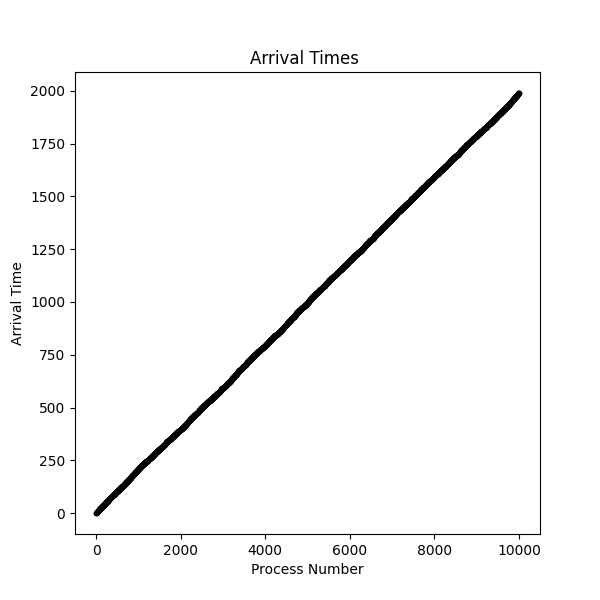
\includegraphics{images/arrival_times.png}
    \caption{Arrival Times of the Jobs}
    \label{Arrival Times of the Jobs}
    \\
The arrival times increase linearly with time.\\
\end{figure}

% INTERARRIVAL TIMES
\begin{figure}
    \centering
    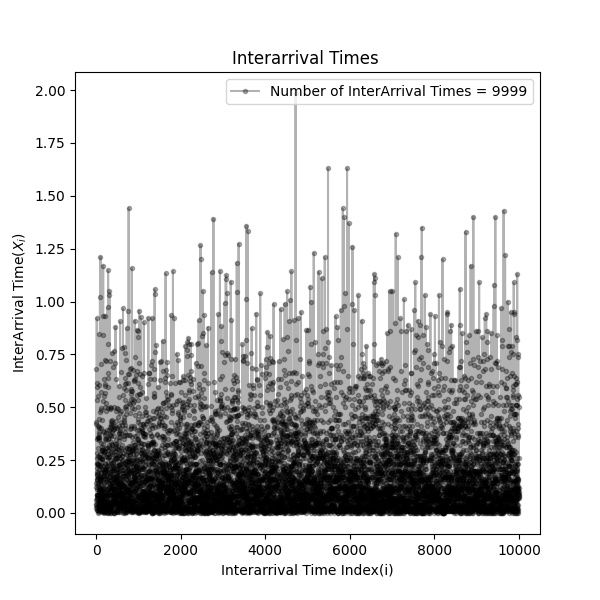
\includegraphics{images/interarrival1.png}
    \caption{Interarrival Times}
    \label{Arrival Times of the Jobs}
\end{figure}
\begin{figure}
    \centering
    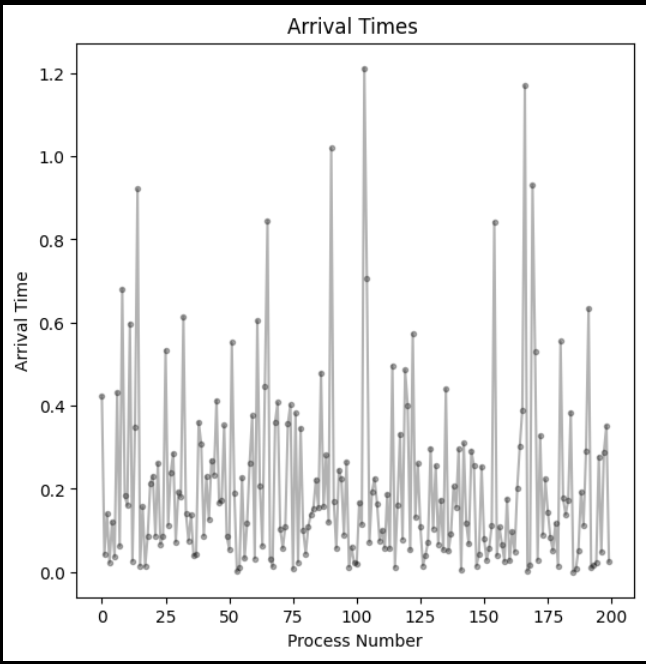
\includegraphics[width=1\linewidth]{images/interarrival2.png}
    \caption{Your Image Caption}
    \label{InterArrival Times of the Processes}
    \\
Clearly, the interarrival times are independent of eachother.\\
\end{figure}


% MEAN SOJOURN TIME
\begin{figure}
    \centering
    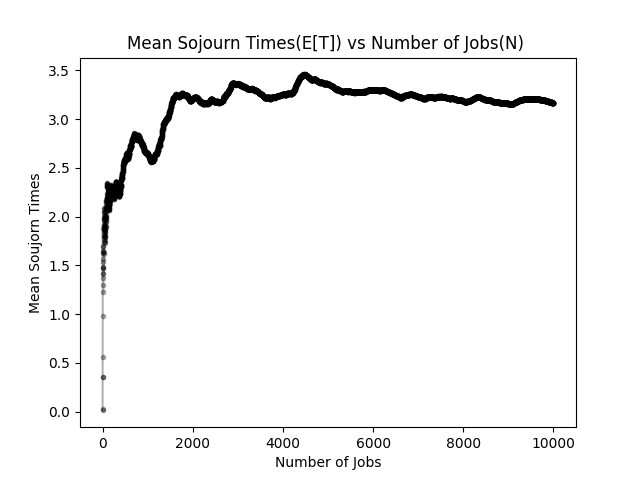
\includegraphics{images/mean_sojourn_times.png}
    \caption{E[T] vs N}
    \label{Mean Sojourn Time vs N}
Mean Sojourn Time converges to the the value 3.16 as number of jobs arrived increases.\\
\end{figure}

% VERIFICATION OF LITTLE LAW
\begin{figure}
    \centering
    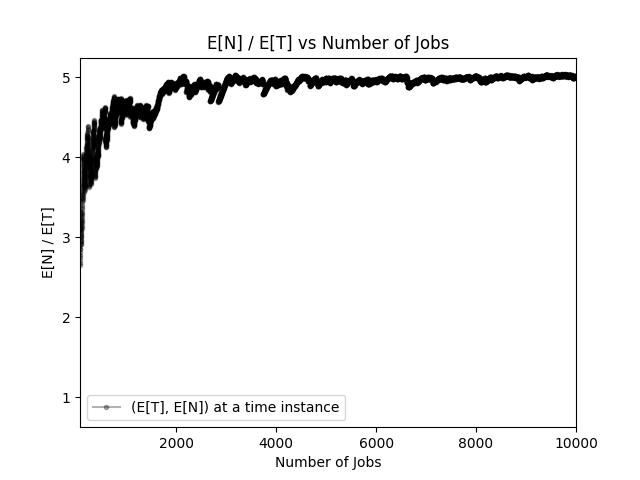
\includegraphics{images/littles_law_verification.png}
    \caption{Verification of Little's Law}
    \label{E[N]/E[T] vs N}
Little's Law is verified by the above plot as when the number of jobs arrived increases, the ratio 
$$ E[N]/E[T]$$
converges to $\lambda$ \\
\end{figure}
% BLOCKING PROBABILITY
\begin{figure}
    \centering
    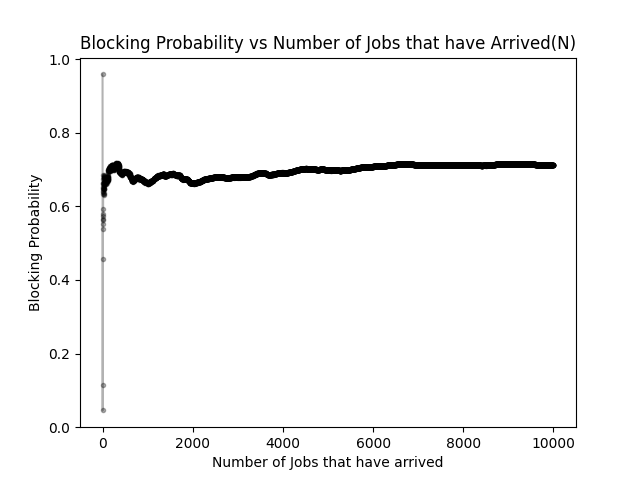
\includegraphics{images/blocking_probability.png}
    \caption{Blocking Probability vs Number of Jobs arrived(N)}
    \label{Blocking Probability vs N}
\\
The Blocking Probability stagnates to 0.70. Notice that the Blocking Probability does not depend on number of jobs that have arrived.
\end{figure}
\end{document}

